%%% In this section, you will describe all of the various artifacts that you will generate and maintain during the project life cycle. Describe the purpose of each item below, how the content will be generated, where it will be stored, how often it will be updated, etc. Replace the default text for each section with your own description. Reword this paragraph as appropriate.

\subsection{Major Documentation Deliverables}

\subsubsection{Project Charter}

This document will be updated a total of three times. Once towards the beginning of senior design 1, the initial delivery date is October 3rd 2018. The second time will be at the end of senior design 1 and the final version will be delivered towards the end of senior design 2.

\subsubsection{System Requirements Specification}
System Requirements Specification is maintained and updated as the team goes through options and weighs cost and risk. Initial version to be done by sprint 2. Final version to be done by sprint 8.

\subsubsection{Architectural Design Specification}
Architectural Design Specification is maintained and updated as the team makes changes to the design. Initial version to be done by sprint 3. Final version to be done by sprint 8.

\subsubsection{Detailed Design Specification}
Detailed Design Specification is maintained and updated as the team makes changes to the design. Initial version to be done by sprint 5. Final version to be done by sprint 8.

\subsection{Recurring Sprint Items}


\subsubsection{Product Backlog}
Backlog items are voted among the team and added through a majority vote. Items will be prioritized based on how it can meet the requirements for the product, such as a camera. Sprint backlogs will be documented on trello.

\subsubsection{Sprint Planning}
Sprint duration of 2 weeks each. Total of 8 sprints.

\subsubsection{Sprint Goal}
Sprint goals are decided by the team and is determined by what has not been completed the previous sprint and what needs to be complete.

\subsubsection{Sprint Backlog}
Backlog items are voted among the team and added through a majority vote. Sprint backlogs will be documented on trello.

\subsubsection{Task Breakdown}
Team members will claim tasks for themselves with the knowledge and agreement of the rest of the team.  The product owner will not have final say over task delegation.  Time will documented in individual sprints.

\subsubsection{Sprint Burndown Charts}
The team will be mutually responsible for the charts.  The format shall be an x,y line graph.  Slack plugin will be used.

\begin{figure}[h!]
    \centering
    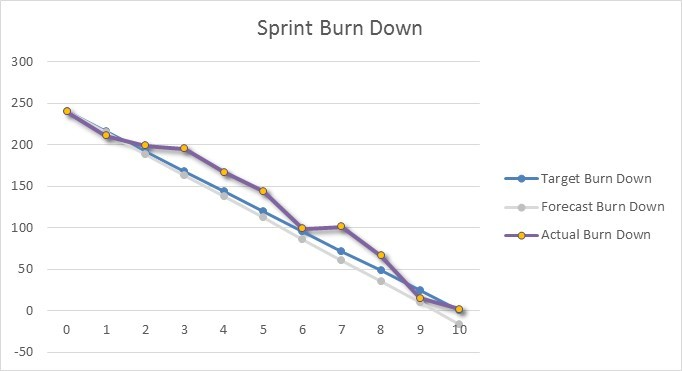
\includegraphics[width=0.7\textwidth]{images/burndownchart}
    \caption{Example sprint burn down chart}
\end{figure}

\subsubsection{Sprint Retrospective}
A meeting after each due sprint will be held immediately after class.  The documentation will be done in the respective engineering notebooks and presentation slides.

\subsubsection{Individual Status Reports}
Whenever a work session is finished, a report will be issued specifying the current progress of assigned tasks.

\subsubsection{Engineering Notebooks}
How often will the engineering notebook be updated, at a minimum, by each team member? What is the minimum amount of pages that will be completed for each interval, and how long will that interval be? How will the team keep each member accountable? Who will sign of as a "witness" for each ENB page?

\subsection{Closeout Materials}

\subsubsection{System Prototype}
The system itself, plus a raspberry pi and camera system, plus a mounting device.  Details of mounting device to be determined.

\subsubsection{Project Poster}
The poster is currently not a prioritized task.  Should it be so in the future, dimensions will be decided upon by the team member assigned this task.

\subsubsection{Web Page}
We will have a web page to provide instructions on how to set up the device and include a demonstration video of how the device works including any important information the user may need to know while using or setting it up. If our group decides to market our product to sell to people, then we will also allow prospective users to purchase the device at a price determined by our team. The web page will be under construction throughout the developmental sprints, but we would like to have some introductory information regarding what we are doing and how we plan to do it posted before then.

\subsubsection{Demo Video}
In our product demonstration video, we will show off what our product is, how it works, and what we hope to accomplish with it. Included in our demonstration video will be information including, but not limited to, how to set it up, how to use it, what information it will be collecting, and any problems we would like to solve with our product.

\subsubsection{Source Code}
Our team’s code will be managed on a team GitHub account that we each have access to. Each member will clone the directory to their personal machine and will commit changes through each members personal GitHub account. Because our product has market potential, we would like to use a private GitHub repository to prevent members outside of our team from accessing our code.
If we do market our product, the customer should be provided access to execute the code and manage any configuration we allow; otherwise, we will keep our product private.

\subsubsection{Source Code Documentation}
While we are still considering other options, we will most likely use Doxygen to manage our source code documentation. Once we have begun work on the development, we will solidify our choice. This way, we will know exactly which languages we will need support for and we will be able to determine our best choice for documentation. We would like to be able to export the source code to a web format that is browsable by the team. Because of this preference, we have chosen Doxygen as it supports exporting to HTML.

\subsubsection{Hardware Schematics}
Because our product is mostly software-based, we will not have much hardware integration to include. Currently, our plan is to use a camera with an infrared and visible light sensor to track any passing vehicles and mount it along with a Raspberry Pi and any other hardware components inside a case. 

\subsubsection{CAD files}
Our product will likely be housed inside of a 3D printed container. To design the housing for everything, we will use one of the many free 3D modelling software available. STL seems to be the best format to save our 3D designs as, so we will be using it to send to the 3D printer.

\subsubsection{Installation Scripts}
Along with our product, we will provide installation instructions to provide the user with simple installation instructions. Should we decide to implement an auto-installer, we will provide the necessary installation information during the installation phase. We will know more about this part when we begin the software implementation of our product.

\subsubsection{User Manual}
The user will be provided information on how to run and use the product in multiple forms. We will allow the user to access our user manual through our web page, which will also contain an installation and demonstration video. 
Along with this, we will provide an offline version of our user manual included with the software or packaged with the product itself. Should the user need any help setting it up, we hope to provide a help page included in the user manual and on the website.